\section{RePair}
\label{sec:method}
\begin{figure}[t]
\centering
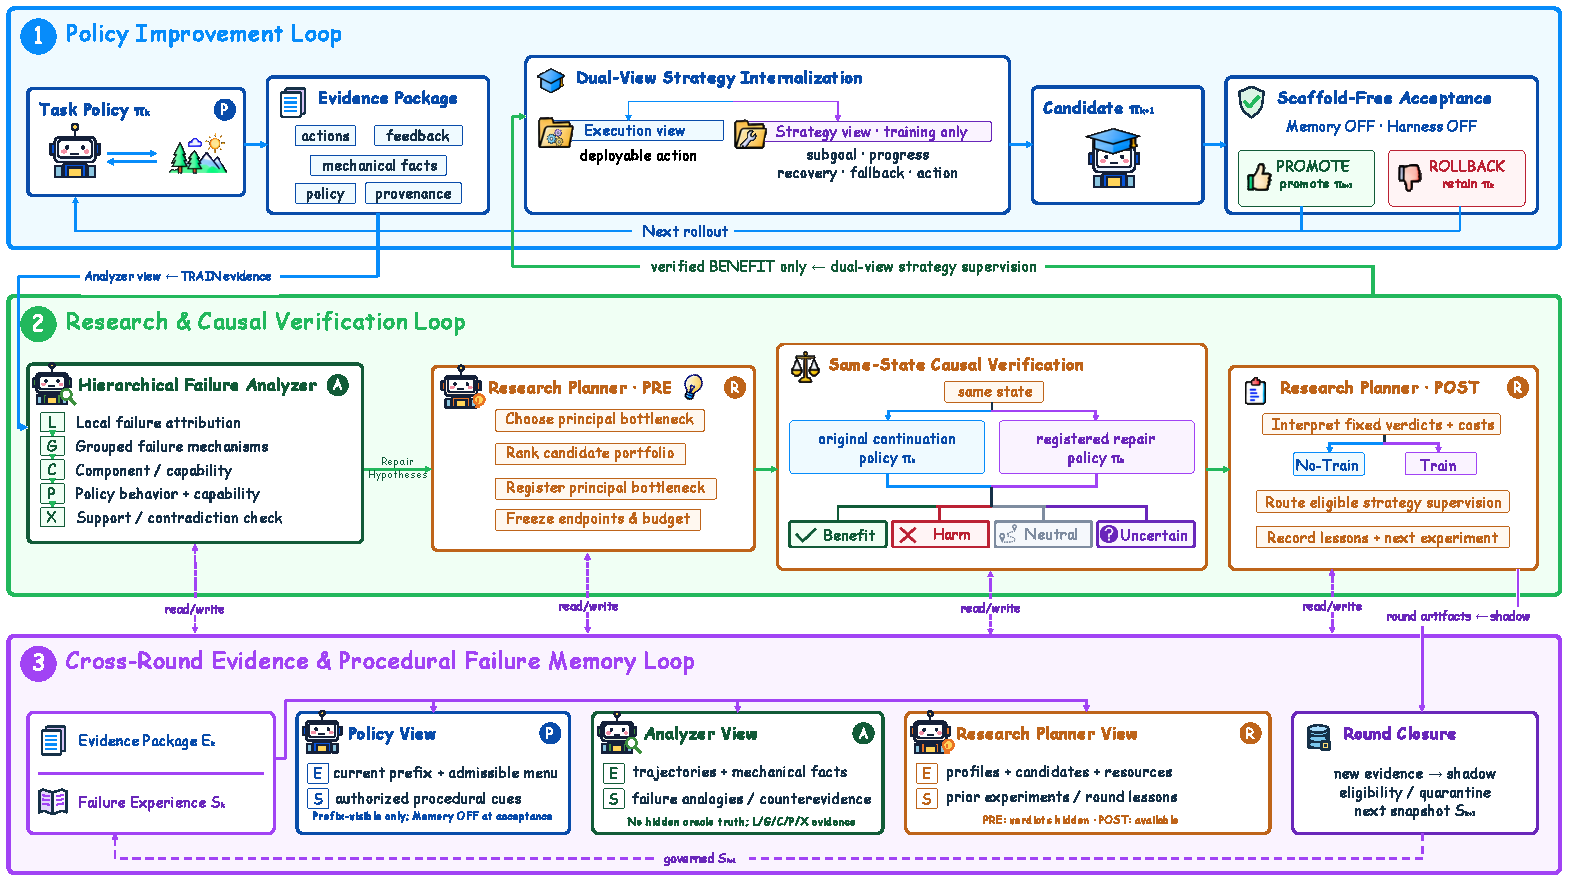
\includegraphics[width=\linewidth]{figures/repair_overview_cropped.pdf}
\caption{\textbf{RePair in context.} The paper follows the scientific path from failure-derived hypotheses through same-state verification, policy supervision, and scaffold-free acceptance. The research and memory loops support proposal selection and carry completed evidence across rounds; Section~\ref{sec:internalization} defines action-only and dual-view targets from verified evidence.}
\label{fig:framework}
\end{figure}

\method{} treats a repair as an experiment before treating it as supervision.
We follow that repair from its source state through testing, training, and
evaluation. Figure~\ref{fig:framework} shows the surrounding research loop;
Appendix~\ref{app:research} describes its analysis and memory mechanisms.

\subsection{Starting from a Failed Attempt}
\label{sec:setup-formal}
Let $\pi_k$ be the task policy entering round $k$. Its input contains a goal,
current observation, recent executed actions and feedback, and an admissible
action menu. We collect trajectories on the training split and retain their
actions, observations, budgets, and terminal outcomes. Completed task failures
supply the repair candidates; infrastructure incidents have their own
execution records.

Each candidate is tied to a recoverable decision state $x$ and the context
$c(x)$ visible to the policy. The source record fixes the checkpoint,
baseline action, action menu, and remaining budget. Environment-restoration
information stays outside $c(x)$. This distinction lets us restore the
experiment while preserving the information available to the agent.

A useful source state precedes a decision the proposal can change. For
example, continuing to search after the target has been found and searching
before it has been found can require different corrections, even if both
trajectories eventually fail. The source context anchors the proposal to
which subgoal is still active and what the agent has already observed.
This makes the unit of investigation a decision within a task.

\subsection{Proposing a Repair That Can Be Tested}
\label{sec:proposal}
The research models inspect a failed trajectory, connect local errors with
recurring failure patterns, and consult earlier repairs and counterexamples.
A planner chooses a principal bottleneck and a small portfolio of tests.
Each proposal specifies a source state, an executable repair $r$, and a
compact strategy describing its subgoal, expected progress, and recovery
conditions. The intervention is an action or a bounded program with conditions
grounded in visible observations and explicit termination rules. Earlier rounds use one action or an
option of at most four actions; the later validation uses ordered guarded
phases within the same remaining environment budget. Its payload, strategy description,
endpoint, and budget are fixed before the environment test.

The researcher receives trajectory observations and mechanical execution
facts, including admissible actions and feedback. It can reason about
search, subgoal transitions, prerequisites, or recovery, but the proposal
must identify how to test that reasoning in the environment. Hidden
restoration state remains with the verifier. This division lets the
research model suggest a high-level strategy while the environment
determines whether its executable realization helps.

This makes the proposal concrete. A suggestion to ``search more carefully''
becomes a particular action or option at a particular state. Related failures
help the researcher distinguish an isolated invalid action from a recurring
problem, such as continuing an exhausted search. Historical experience
supplies possible next steps and the conditions under which they previously
helped. These sources guide where to spend the test budget; current paired
rollouts measure the effect on $\pi_k$.

Research within a round reads a fixed history snapshot. The proposal can
use a lesson from an earlier round, but its action and strategy are settled
before the current outcomes are revealed. Completed outcomes then become
historical evidence for the next round (Appendix~\ref{app:views}). This
allows research to accumulate experience while keeping each proposed
intervention tied to a specific test.

\subsection{Returning to the Same State}
\label{sec:verification}
For a candidate $(x,r)$, we restore $x$ twice. Branch $F_0$ executes the
registered baseline action $a_0$; branch $F_1$ executes the repair. If the task remains unfinished, the same frozen policy $\pi_k$ supplies
subsequent decisions:
\begin{equation}
\begin{aligned}
F_0 &: x\xrightarrow{a_0}x'_0\xrightarrow{\pi_k}Y^{(0)},\\
F_1 &: x\xrightarrow{r}x'_1\xrightarrow{\pi_k}Y^{(1)}.
\end{aligned}
\label{eq:branches}
\end{equation}
Here $Y^{(b)}\in\{0,1\}$ is terminal task success. We repeat the paired
comparison five times. Each pair shares the starting state and visible
context, checkpoint, base prompt interface, memory snapshot, remaining budget, and
paired seed protocol. In the later strategy validation, $r$ also includes
a registered strategy cue on F1 continuation calls; the treatment is the
program and cue together, not an isolated action change. The baseline is a fresh policy continuation and can succeed
even though the source episode failed.

After the intervention the branches are free to diverge; that divergence
is precisely what the repair is meant to cause. Every intervention action
consumes the remaining interaction budget. For an option, the test covers
the complete registered option, with admissibility checked at each reached
state. Across repetitions, the joint $F_0/F_1$ outcomes describe the local,
policy-conditioned effect of the proposed change. Appendix~\ref{app:restoration}
gives the restoration and execution checks.

Keeping the continuation policy fixed is central to this test. Replacing it
with a stronger teacher asks whether the teacher can finish after the
intervention. When continuation is needed, using $\pi_k$ tests whether the learner can
use the state reached by the intervention. If the program already reaches
success, no policy continuation is required; we explicitly count this case. In the cabinet
example, exposing an object is useful only to the extent that the remaining
policy can turn that opportunity into task completion within the budget.
Intermediate progress helps explain the branches; terminal success supplies
the effect label.

\subsection{Selecting Repairs for Learning}
\label{sec:eligibility}
An independent verifier reads the paired outcomes. A candidate receives
\emph{Benefit} when at least four of the five valid pairs change failure to
success and none changes success to failure. The symmetric rule gives
\emph{Harm}. Stable success in both branches and stable failure in both
branches give two neutral outcomes; other complete results are uncertain.
We use these repetitions to assess stability at the selected state;
Appendix~\ref{app:labels} gives the exact counts and treatment of incomplete tests.

Let $\mathcal I_k$ contain completed interventions whose source and training
records agree with the executed test. Positive supervision is the Benefit subset:
\begin{equation}
\mathcal D_k^+=\{i\in\mathcal I_k:L_i=\Benefit\}.
\label{eq:eligibility}
\end{equation}
A change that repeatedly helps the current policy thus becomes a candidate
lesson. The verifier selects on its executed effect; the associated strategy
remains the description fixed before testing.

The remaining outcomes also inform research. Repeated success in both
branches suggests that this correction is unnecessary under the tested
conditions. Repeated failure leaves an unresolved difficulty, and a harmful
intervention supplies a counterexample to the proposal. The planner uses
these outcomes and their costs to choose TRAIN or NO-TRAIN and to guide
later tests. This gives negative experiments a role without putting them
in the positive-supervision set.

\subsection{Learning an Action or Learning Its Strategy}
\label{sec:internalization}
A verified intervention tells us which decision helped. We now ask how to
teach it. A historical data-path audit made this question concrete: an
action-only materialization retained the chosen actions as targets while
richer strategy information remained upstream
(Appendix~\ref{app:historical}). We therefore make that information an explicit auxiliary prediction
target. The action-only formulation below defines the corresponding
control; the completed update in this study uses dual views.

\emph{Action-only} supervision uses the deployment context $c_i$ and the
target $a_i$, serialized as \texttt{\{"action":"..."\}}. Let $c_i^s$
denote the same legal source context with a fixed training-only instruction.
\emph{Dual-view} supervision keeps the action examples and adds a strategy view:
\begin{equation}
\begin{aligned}
\mathcal T_{\mathrm{action}}&=\{(c_i,a_i):i\in\mathcal D_k^+\},\\
\mathcal T_{\mathrm{dual}}&=\mathcal T_{\mathrm{action}}\cup
\{(c_i^s,s_i):i\in\mathcal D_k^+\}.
\end{aligned}
\label{eq:training-views}
\end{equation}
The strategy instruction requests a compact response $s_i$ with
the bottleneck, subgoal, expected event and state change, progress criterion,
recovery trigger, fallback condition, and action. These fields relate a
choice to the task: the subgoal says what it is meant to accomplish, the
progress criterion says what to check next, and recovery conditions say
when to change course. Table~\ref{tab:views-example} illustrates the
information added to an action target.
\begin{table}[H]
\caption{\textbf{What each training view teaches.} Schematic example:
the agent is looking for an object beside a closed cabinet, and
\texttt{open cabinet 1} is admissible. The auxiliary view adds prospective
task information to the same action. This illustrates target content.}
\label{tab:views-example}
\centering\small
\begin{tabularx}{\linewidth}{@{}L{1.10in}X@{}}
\toprule
View & Supervised content\\
\midrule
Execution & \texttt{\{"action":"open cabinet 1"\}}\\
Strategy & Subgoal: inspect the cabinet. Expected progress: its contents
become visible. Check: whether the target is present. Recovery/fallback:
if it is absent, continue the search elsewhere. Action:
\texttt{open cabinet 1}.\\
\bottomrule
\end{tabularx}
\end{table}


The response uses the strategy registered before verification. Expected
progress is prospective: it states what to look for in subsequent feedback.
Realized future outcomes, rewards, and effect labels are excluded from
prediction targets. In the completed update, each source contributes its initial action and
one strategy response. The later actions of a successful intervention are
not expanded into additional execution-view examples. This distinction
between verified program coverage and supervised action coverage matters
for interpreting transfer.

The two views update the same policy weights through supervised
assistant-token loss. Prompt tokens are masked; the auxiliary response
makes the strategy itself a prediction target. The native-label check
confirms that both action and substantive strategy tokens contribute to
that loss. The fixed auxiliary instruction gives this training task its
own output format while the original parser continues to accept exactly
one action field. Evaluation uses the execution view directly, with no
strategy-generation step or additional research-model call.

A controlled representation comparison would start both conditions from
the same parent and evidence, and include an equal-compute action-only
control. Those controls are not completed here. We report the executed
dual-view labels, tokens, and optimizer steps in
Appendix~\ref{app:training-details}; the observed parent--candidate change
therefore measures this update as a whole.

\subsection{Removing the Assistance}
\label{sec:iteration}
The final test belongs to the policy. We remove external failure memory and
repair takeover and compare candidate $\pi'$ with parent $\pi$ under the
original action interface. For task $t$ and seed $j$, let $Y_{tj}(\pi)$ denote
terminal success in this scaffold-free setting. We measure
\begin{equation}
\begin{aligned}
\widehat{\SR}_{\mathcal D}(\pi)
&=\frac{1}{|\mathcal D|}\sum_{t\in\mathcal D}
\frac{1}{J_{\mathrm{eval}}}\sum_{j=1}^{J_{\mathrm{eval}}}Y_{tj}(\pi),\\
\Delta^{\mathcal D}_{\mathrm{policy}}(\pi',\pi)
&=\widehat{\SR}_{\mathcal D}(\pi')-\widehat{\SR}_{\mathcal D}(\pi).
\end{aligned}
\label{eq:policy-eval}
\end{equation}
The goal, observations, ordinary within-task history, admissible menu, and
strict action parser remain available to both policies. Evaluation starts
at each task's initial state, so the learned model also has to reach useful
decisions without being placed at a selected failure point. This extends
the local intervention test to complete task behavior.

During the improvement loop, an independent predeclared acceptance rule
compares candidate and parent on training-side selection tasks, after
integrity checks. In the final validation, success count is primary; ties
use the mean terminal fraction of satisfied goal conditions, evaluated
outside the policy input. No clear improvement retains the parent. A NO-TRAIN decision retains the
parent. The retained policy collects fresh failures for the next round, and
completed research updates the next history snapshot. The final seen and
unseen benchmark sets are evaluated after selection; their scores stay
outside this adaptive loop. Appendix~\ref{app:research} specifies the full
return from one round to the next.
